\documentclass[a4paper,10pt]{article}
\usepackage[french]{babel}
\usepackage[utf8]{inputenc}
\usepackage[left=2.5cm,top=2cm,right=2.5cm,nohead,nofoot]{geometry}
\usepackage{url}
\usepackage{graphicx}
\usepackage{pbox}
\usepackage{float}
\usepackage[colorinlistoftodos]{todonotes}
\usepackage{hyperref}

\linespread{1.1}

%\setcounter{section}{-1}

\begin{document}

\begin{titlepage}
\begin{center}
\textbf{\textsc{UNIVERSIT\'E DE MONTR\'EAL}}\\
%\textbf{\textsc{Faculté des Sciences}}\\
%\textbf{\textsc{Département d'Informatique}}
\vfill{}\vfill{}
\begin{center}{\Huge Rapport : TP2 - Classification de textes}\end{center}{\Huge \par}
\begin{center}{\large Pierre Gérard}\end{center}{\Huge \par}
\vfill{}\vfill{} \vfill{}
\begin{center}{\large \textbf{IFT 3335 Intelligence artificielle: Introduction}}\hfill{\\Jian-Yun Nie, William Lechelle}\end{center}{\large\par}
\vfill{}\vfill{}\enlargethispage{3cm}
\textbf{Année académique 2015~-~2016}
\end{center}
\end{titlepage}

%\begin{abstract}
%Ce rapport présente ...
%\end{abstract}


%\tableofcontents

%\pagebreak

\section{Méthode de base}

Il est demandé, pour trouver un point de base pour effectuer des comparaisons d'analyser la classification avec le classifieur Bayes Naif et une validation croisé 10-fold.

\subsection{Résultats expérimentaux}

\subsubsection{Reuters-21578}
Pour le sous ensemble Reuters-21578 avec le classifieur Bayes Naif et une validation croisé 10-fold, on obtient les résultats suivant :
\begin{verbatim}
=== Summary ===
Correctly Classified Instances        3235               79.3087 %
Incorrectly Classified Instances       844               20.6913 %     
=== Detailed Accuracy By Class ===
               TP Rate   FP Rate   Precision   Recall  F-Measure   ROC Area  Class
                 0.765     0.113      0.858     0.765     0.809      0.925    Neg-
                 0.843     0.102      0.791     0.843     0.816      0.929    Pos-earn
                 0.429     0          0.6       0.429     0.5        0.968    Pos-housing
                 0.805     0.075      0.72      0.805     0.76       0.949    Pos-acq
                 0.629     0.013      0.297     0.629     0.404      0.912    Pos-coffee
                 0.471     0.003      0.571     0.471     0.516      0.939    Pos-gold
                 0.75      0          0.6       0.75      0.667      0.949    Pos-heat
Weighted Avg.    0.793     0.1        0.802     0.793     0.795      0.931
\end{verbatim}

\subsubsection{Ohsumed}
Pour le sous ensemble Ohsumed, on obtient les résultats suivant :
\begin{verbatim}
=== Summary ===
Correctly Classified Instances        1917               35.632  %
Incorrectly Classified Instances      3463               64.368  %    
=== Detailed Accuracy By Class ===
               TP Rate   FP Rate   Precision   Recall  F-Measure   ROC Area  Class
                 0.174     0.074      0.74      0.174     0.282      0.696    Neg-
                 0.511     0.114      0.166     0.511     0.251      0.771    Pos-Hyperplasia
                 0.349     0.023      0.193     0.349     0.249      0.724    Pos-Mitosis
                 0.5       0.055      0.43      0.5       0.463      0.797    Pos-Necrosis
                 0.698     0.245      0.059     0.698     0.109      0.853    Pos-Pediatrics
                 0.376     0.028      0.653     0.376     0.477      0.797    Pos-Pregnancy
                 0.779     0.196      0.45      0.779     0.571      0.849    Pos-Rats
Weighted Avg.    0.356     0.093      0.608     0.356     0.364      0.749
\end{verbatim}

\subsection{Discussion}

Pour analyser les résultats, définissons quelques concepts :
\begin{itemize}
	\item Validation croisé : Pour éviter le sur-apprentissage (apprendre "par coeur" les données) ont divise l'ensemble d'entrainement en plusieurs parties, une sur laquelle on effectue le calcul de performance de l'apprentissage, les autres sur lequel on effectue l'apprentissage en lui-même. Cependant, en faisant ça on perd des données pour l'apprentissage car une partie est utilisé pour le test. C'est pourquoi on répète cette opération x fois avec un ensemble de test différent a chaque fois. Cela permet de raffiner l'apprentissage a chaque fois.
	\item Erreur de test : L'erreur de test est le pourcentage d'article mal classifié sur l'ensemble de test. On peut considérer cette erreur comme l'erreur de généralisation.
	\item Précision : La précision est le ratio de vrai positif sur la somme du nombre de faux et de vrai positif. En d'autres terme, le ratio de correctement identifié parmis ceux identifié.
	\item Rappel : Le rappel est le ratio de vrai positif sur le nombre d'element de l'ensemble. En d'autres terme, c'est égale au nombre d'articles correctement classifié.
\end{itemize}

Ici, on remarque que NaiveBayes semble classifier avec beaucoup plus de facilité l'ensemble de donnée de Reuters que l'ensemble de donnée Ohsumed.

\todo{bullshiter un peu}

\section{Selection d'attributs}

La selection d'attribut pourrait permettre d'accélérer les algorithme et peut-être améliorer l'apprentissage en éliminant des attributs non pertinent. Regardons son effet :

\subsection{Résultats expérimentaux}

\subsection{Test 1}
Ce test est celui demandé dans l'énoncé. Il consiste a aller dans "Attribute Evaluator", choisir la méthode ChiSquarred, et dans "Search Method" la méthode Ranker qui ordonne les attributs selon leur valeur et en précisant un nombre à garder.
\begin{figure}[H]
	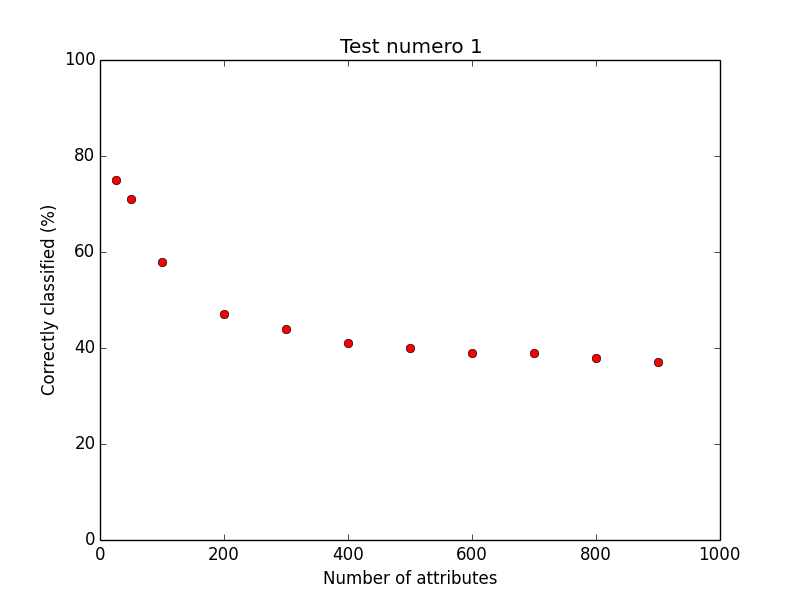
\includegraphics[width=7cm]{images/part2.png} 
	\centering
	\caption{ChiSquarred method with Ohsumed dataset test 1}
	\label{fig:comp}
\end{figure}

\subsection{Test 2}
Ce test consiste a suivre les indications de la documentation Weka concernant la selection d'attribut et la validation croisé. Elle consiste a ne pas pré-sélectionner les attributs, mais à inclure la selection directement dans le classifieur via AttributeSelectedClassifier dans lequel on préciser InfoGainEvaluator, Ranker, et NaiveBayer.

\begin{figure}[H]
	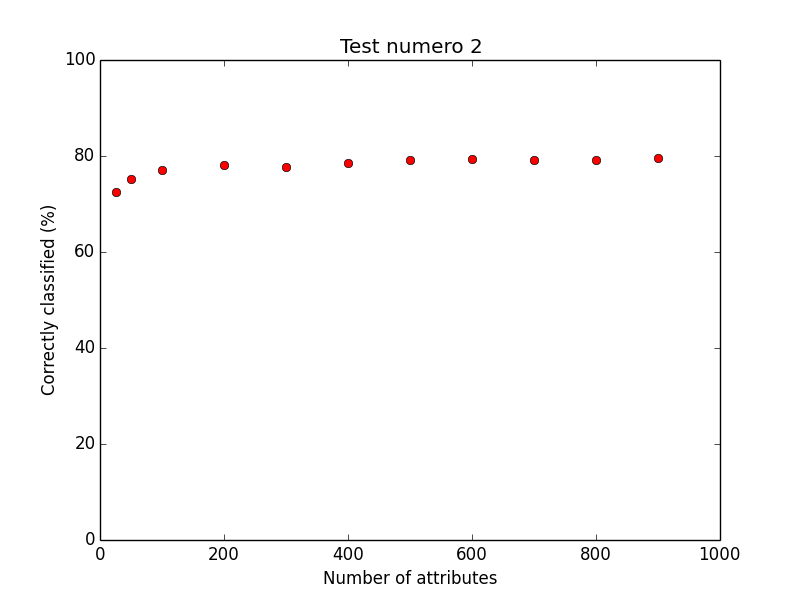
\includegraphics[width=7cm]{images/part2b.png} 
	\centering
	\caption{InfoGain method with Ohsumed dataset test 1}
	\label{fig:comp}
\end{figure}


\subsection{Analyse, discussion et menaces à la validité}

Comme indiqué dans la documentation Weka, la première technique ci-dessus est biaisé, en effet elle évalue la performance de l'algorithme sur les attributs sélectionné qui sont eux-mêmes les plus performant. En d'autres termes, cela veut dire que la performance est évalué sur les attributs qui vont indiqués la meilleur performance.

Le deuxième test montre bien quant à lui la performance de généralisation de l'algorithme après avoir sélectionner des attributs.

On remarque donc que sélectionner une partie des attributs dans les 50 - 80 \% de ceux de départ augmente légèrement la performance de généralisation de l'algorithme. De plus cette selection permet d'accélérer la vitesse d'exécution des algos car ils ne traitent pas dans ce cas la de données "inutiles à la classification".

Pour conclure, on peut dire que sélectionner des attributs est bénéfique. Si on en garde trop, on a du “bruit” qui menace notre apprentissage. Si en garde pas assez, on a une “perte d’information” essentielle qui menacera la performance de généralisation de l'algorithme.

\section{Stemming}

Le "stemming" est un processus qui permet de réduire l'ensemble des dérivé d'un mot à sa forme de base. Cela peut sembler une bonne idée car cela permettrait de rendre identique des termes présentant la même idée. Exemple : "mangeais, manger, mangera, ..". Mais cela peut aussi engendrer une perte d'information; par exemple si on transforme "mangeais" en "manger", on perd la notion que cela était une action passé.

\subsection{Résultats expérimentaux}

Pour tester l'utilité du stemming, réalisons une expérience empirique pour différents algorithme et nombre d'attributs retenu et cela pour les deux ensembles de données.

Regardons le pourcentage d'éléments bien classifié:
\begin{center}
\begin{tabular}{ |c|c|c| } 
 \hline
  & Sans stemming & Avec stemming \\ 
 \hline
 Ohsumed NaiveBayes 1000 attributs 10-fold  & 35.6\% & 37.9\% \\ 
 Ohsumed NaiveBayes 300 attributs 10-fold  & 44.1\% & 45.4\% \\ 
 Ohsumed J48 300 attributs 3-fold & 76.4\% & 77.5\% \\ 
 Ohsumed AdaBoost 300 attributs 10-fold & 62.5\% & 66.9\% \\
 \hline
 Reuters NaiveBayes 1000 attributs 10-fold & 79.3\% & 79.7\% \\
 Reuters NaiveBayes 300 attributs 10-fold  & 78.6\% & 78.5\% \\ 
 Reuters J48 300 attributs 3-fold & 87.4\% & 86.9\% \\ 
 Reuters AdaBoost 300 attributs 10-fold & 70.1\% & 70.1\% \\ 
 Reuters AdaBoost 1000 attributs 10-fold & 70.0\% & 70.0\% \\ 
 \hline
\end{tabular}
\end{center}
La précision n'est pas indiqué ici, elle varie de manière similaire au rappel.

\subsection{Analyse et discussion}
Pour Ohsumed, on remarque que, dans la plupart des cas, le nombre d'attribut bien classifié augmente lorsqu'on utilise la technique de stemming. 

Pour Reuters, on remarque que le stemming n'a pas grande influence sur les résultats.
\todo{discutons}

\section{Evaluation des algos}

\subsection{Résultats expérimentaux}

\subsubsection{Reuters-21578}

\begin{center}
\begin{tabular}{ |c|c|c|c|c| } 
 \hline
  & \pbox{20cm}{Classification \\ correcte} &  \pbox{20cm}{Classification \\ incorrecte} & Précision \\ 
 \hline
 NaiveBayes 1000 attributs 10-fold  & 79.31\% & 20.69\% & 0.8\\ 
 J48 1000 attributs 10-fold  & 87.77\% & 12.23\% & 0.88\\ 
 SMO 1000 attributs 10-fold  & 92.44\% & 7.56\% & 0.92\\ 
 Réseau de neurones (3 layers) 1000 attributs 4-fold  & 57.8\% & 42.2\% & 0.46 \\ 
 Réseau de neurones (5 layers) 1000 attributs 4-fold  & 57.8\% & 42.2\% & 0.46\\ 
 Réseau de neurones (10 layers) 1000 attributs 4-fold  & 84.04\% & 15.96\% & 0.84\\ 
 Réseau de neurones (30 layers) 1000 attributs 4-fold  & 86.1\% & 13.9\% & 0.85\\  
 \hline
\end{tabular}
\end{center}

\subsubsection{Ohsumed}

\begin{center}
\begin{tabular}{ |c|c|c|c| } 
 \hline
  & \pbox{20cm}{Classification \\ correcte} &  \pbox{20cm}{Classification \\ incorrecte} & Précision \\ 
 \hline
 NaiveBayes 1000 attributs 10-fold  & 35.6\% & 64.4\% & 0.6 \\ 
 J48 1000 attributs 10-fold  & 76.0\% & 24.0\% & 0.75 \\ 
 SMO 1000 attributs 10-fold  & 67.9\% & 32.1\% & 0.67 \\ 
 Réseau de neurones (3 layers) 1000 attributs 4-fold  & 54.8\% & 45.2\% & 0.3 \\ 
 Réseau de neurones (5 layers) 1000 attributs 4-fold  & 54.8\% & 45.2\% & 0.3 \\ 
 Réseau de neurones (10 layers) 1000 attributs 4-fold  & 60.5\% & 39.5\% & 0.45 \\ 
 Réseau de neurones (30 layers) 1000 attributs 4-fold  & 54.8\% & 45.2\% & 0.3 \\  
 \hline
\end{tabular}
\end{center}

\subsection{Discussion}

\todo{discussion}

\section{Exploration}

Nous allons désormais exploré les différentes possibilités du logiciel et les différents algorithmes parmis ceux généralement prescrit pour la classification de document.



%\section{Introduction}

%\section{Etat de l'art}

%\section{Méthode expérimentale}

%\section{Résultats expérimentaux}

%\section{Discussion}

%\section{Conclusion}

\end{document}
